In this chapter we describe the design of a Convolutional Neural Network that can process thermal images and predict what object they contain.
The workflow that we followed will largely be a combination of the workflows presented in Figures \ref{ml_workflow} and \ref{micro_workflow}.

We first had to set concrete objectives, while keeping in consideration various constraints.
The tools and development environment that were used in the process are then described. 
The methods of dataset creation are described afterwards: first, the dataset that was created by Arribada Initiative, then the dataset provided by us. 

We then explored both datasets, analysed different class representations, and decided if they were appropriate for accomplishing the objectives that we set earlier.

In the image preprocessing phase we imported images and connected them with metadata that was parsed from the Excel database.
We analysed the dataset, split it into different sets, and applied image correction procedures.
We then decided on a rough CNN architecture with variable hyperparameters, and ran a random search algorithm, which searched for the best performing models based on accuracy.

We finish this chapter by going through the same design process again, but this time using tools provided by Edge Impulse.


\section{ Model objectives}\label{model_obj}


The accuracy of our early warning system should be equal or similar to the one of the human observers, no matter if it is operating in daytime or night time.
Although the system will be placed on paths that are traversed regularly by elephants, they are not the only possible objects that can appear on the taken thermal images.
Humans and various livestock, such as goats and cows, could also be photographed.
Reporting false positives should be avoided, which means that the system should not label a human or a livestock animal incorrectly as an elephant.
At the same time, false negatives also need to be avoided, as an elephant could pass the system undetected.
These kinds of mistakes could undermine the community's confidence in the early warning system and defeat the purpose.
This means that, besides elephant detection, we should also focus on classifying humans and livestock correctly, while providing a nature/random class for all other unexpected objects or simply images of nature.

It would be beneficial if the thermal camera could take several images of the same object in a short time, thus increasing the confidence of the computed label of the object.
However, this is constrained by the image processing time and the camera's field of view.
The thermal camera FLIR Lepton has a horizontal field of view of 57 degrees.
The closer an object passes by a thermal camera, the quicker it traverses the camera's field of view, thus giving the camera less time for capture.
This problem can be solved by minimising the execution time of the ML model, or by placing the early warning system in a position that is several metres away from the expected elephant's path.
As the latter option might not always be possible, we should strive to keep the whole image processing time as short as possible.

Finally, as our Neural Network has to run on a microcontroller and not on a computer or a server, we have to keep it lightweight in terms of memory.
Extra model complexity that brings few percents of accuracy does not matter much if the model is too large to fit on a microcontroller or takes too long to run.

To summarise:

\begin{itemize}
    \item We will create an image classification ML model that will be capable of processing a thermal image and sorting it into one of 4 possible categories: Elephant, human, livestock, and nature/random.
    \item Total image processing time should be as short as possible: we should try to keep it under 1 second.
    \item The model should be small enough to fit on a microcontroller of our choice, while still leaving some space for the application code. The microcontroller of our choice (STM32F767) has 2 \si{\mega\byte} of flash memory, so the model size should be smaller than that.
\end{itemize}


\section{ Tools and development environment}

All of the work connected with image preparation and ML model creation was done in Python 3.6, Numpy was used for image preprocessing, Pandas for Excel database manipulation, and Matplotlib for plot generation.
The Neural Networks were designed in TensorFlow 2.4, using Keras high-level API and a Keras Tuner model was used for the hyperparameter search.

As training Neural Networks is a computationally demanding process, it would not be feasible to do it on a personal laptop.
Amazon's Elastic Compute Cloud web service was used instead.
Elastic Compute Cloud, or EC2, enables users to create an instance of a server in a cloud with a specified amount of processing power and memory.
Some instances come with dedicated software modules and dedicated graphics cards for an extra boost in performance.
We created an instance of a Linux server that came with TensorFlow, Numpy, and other libraries pre-installed.
Interaction with servers was done one command line through the SSH protocol.

Instead of writing Python scripts and executing them through the command line, we used Juptyer Notebook. 
Juptyer Notebook is a web-based application that can run programs that are a mix of code, explanatory text, and computer output.
Users can divide code into segments, which can be executed separately, and visual output from modules such as Matplotlib is also supported.
To use Juptyer Notebook on our cloud instance, we had to install and run it.
We could then access the web service simply through a web browser by writing the IP address of the server, followed by the default Juptyer Notebook server port, 8888.


\section{ Creating the dataset}

As mentioned in Section \ref{arribada_init}, the major part of the thermal image dataset was provided by the Arribada Initiative\cite{wildlabs-winners}\cite{arribada-assam}.
Images in the dataset came from two different locations: Assam, India, and ZSL Whipsnade Zoo, in the United Kingdom.

Assam served as a testing ground.
The Arribada team positioned two camera traps at two locations that overlook paths commonly used by elephants.
Cameras were built out of Raspberry Pi, a Passive Infrared Sensor (PIR) sensor, an FLIR Lepton 2.5 camera, and batteries, all of which were enclosed in a plastic housing.
The insides of the camera and an example of a deployed camera can be seen in Figure \ref{assam_camera}.

\begin{figure}[ht]
    \begin{subfigure}{0.5\textwidth}
        \centering
        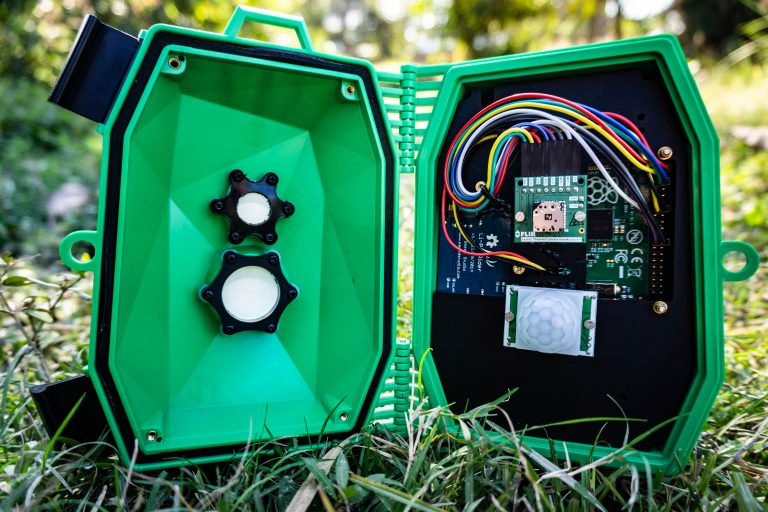
\includegraphics[width=1.0\linewidth, height=5cm]{assam_camera1.jpg} 
    \end{subfigure}
    \begin{subfigure}{0.5\textwidth}
        \centering
        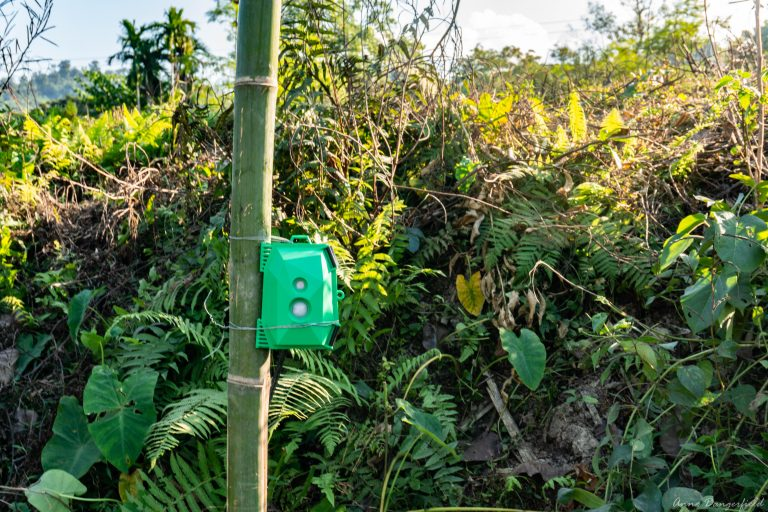
\includegraphics[width=1.0\linewidth, height=5cm]{assam_camera2.jpg}
    \end{subfigure}
    \caption[Camera trap used in Assam, India.]{Camera trap used in Assam, India. Image source: Arribada Initiative\cite{arribada-assam}}
    \label{assam_camera}
\end{figure}

The PIR sensor functioned as a photo trigger: whenever an object passed in front of it, the camera made an image.
This setup provided Arribada with elephant images in real-life scenarios, however, they could not capture elephants in a variety of different conditions. 
It is important to create an image dataset, where the object can be seen in different orientations, distances, angles, and temperature conditions.
Models that were trained on diverse datasets end up being much more robust and, therefore, perform better on never before seen image data, when deployed in real life.

This was accomplished in ZSL Whipsnade Zoo, where they took many images of elephants in a variety of different conditions\cite{dataset_collection}.
With elephants in the enclosure, researchers could move cameras around and get images that were needed.
The PIR sensor trigger approach was dropped in favour of a 5 second time-lapse trigger.
Two cameras were used again, although, one of them now used an FLIR Lepton 3.5 camera with better resolution.

Images of elephants that came from both locations can be seen in Figure \ref{four_elephants}.

\begin{figure}[ht]
    \centering
    \scalebox{.35}{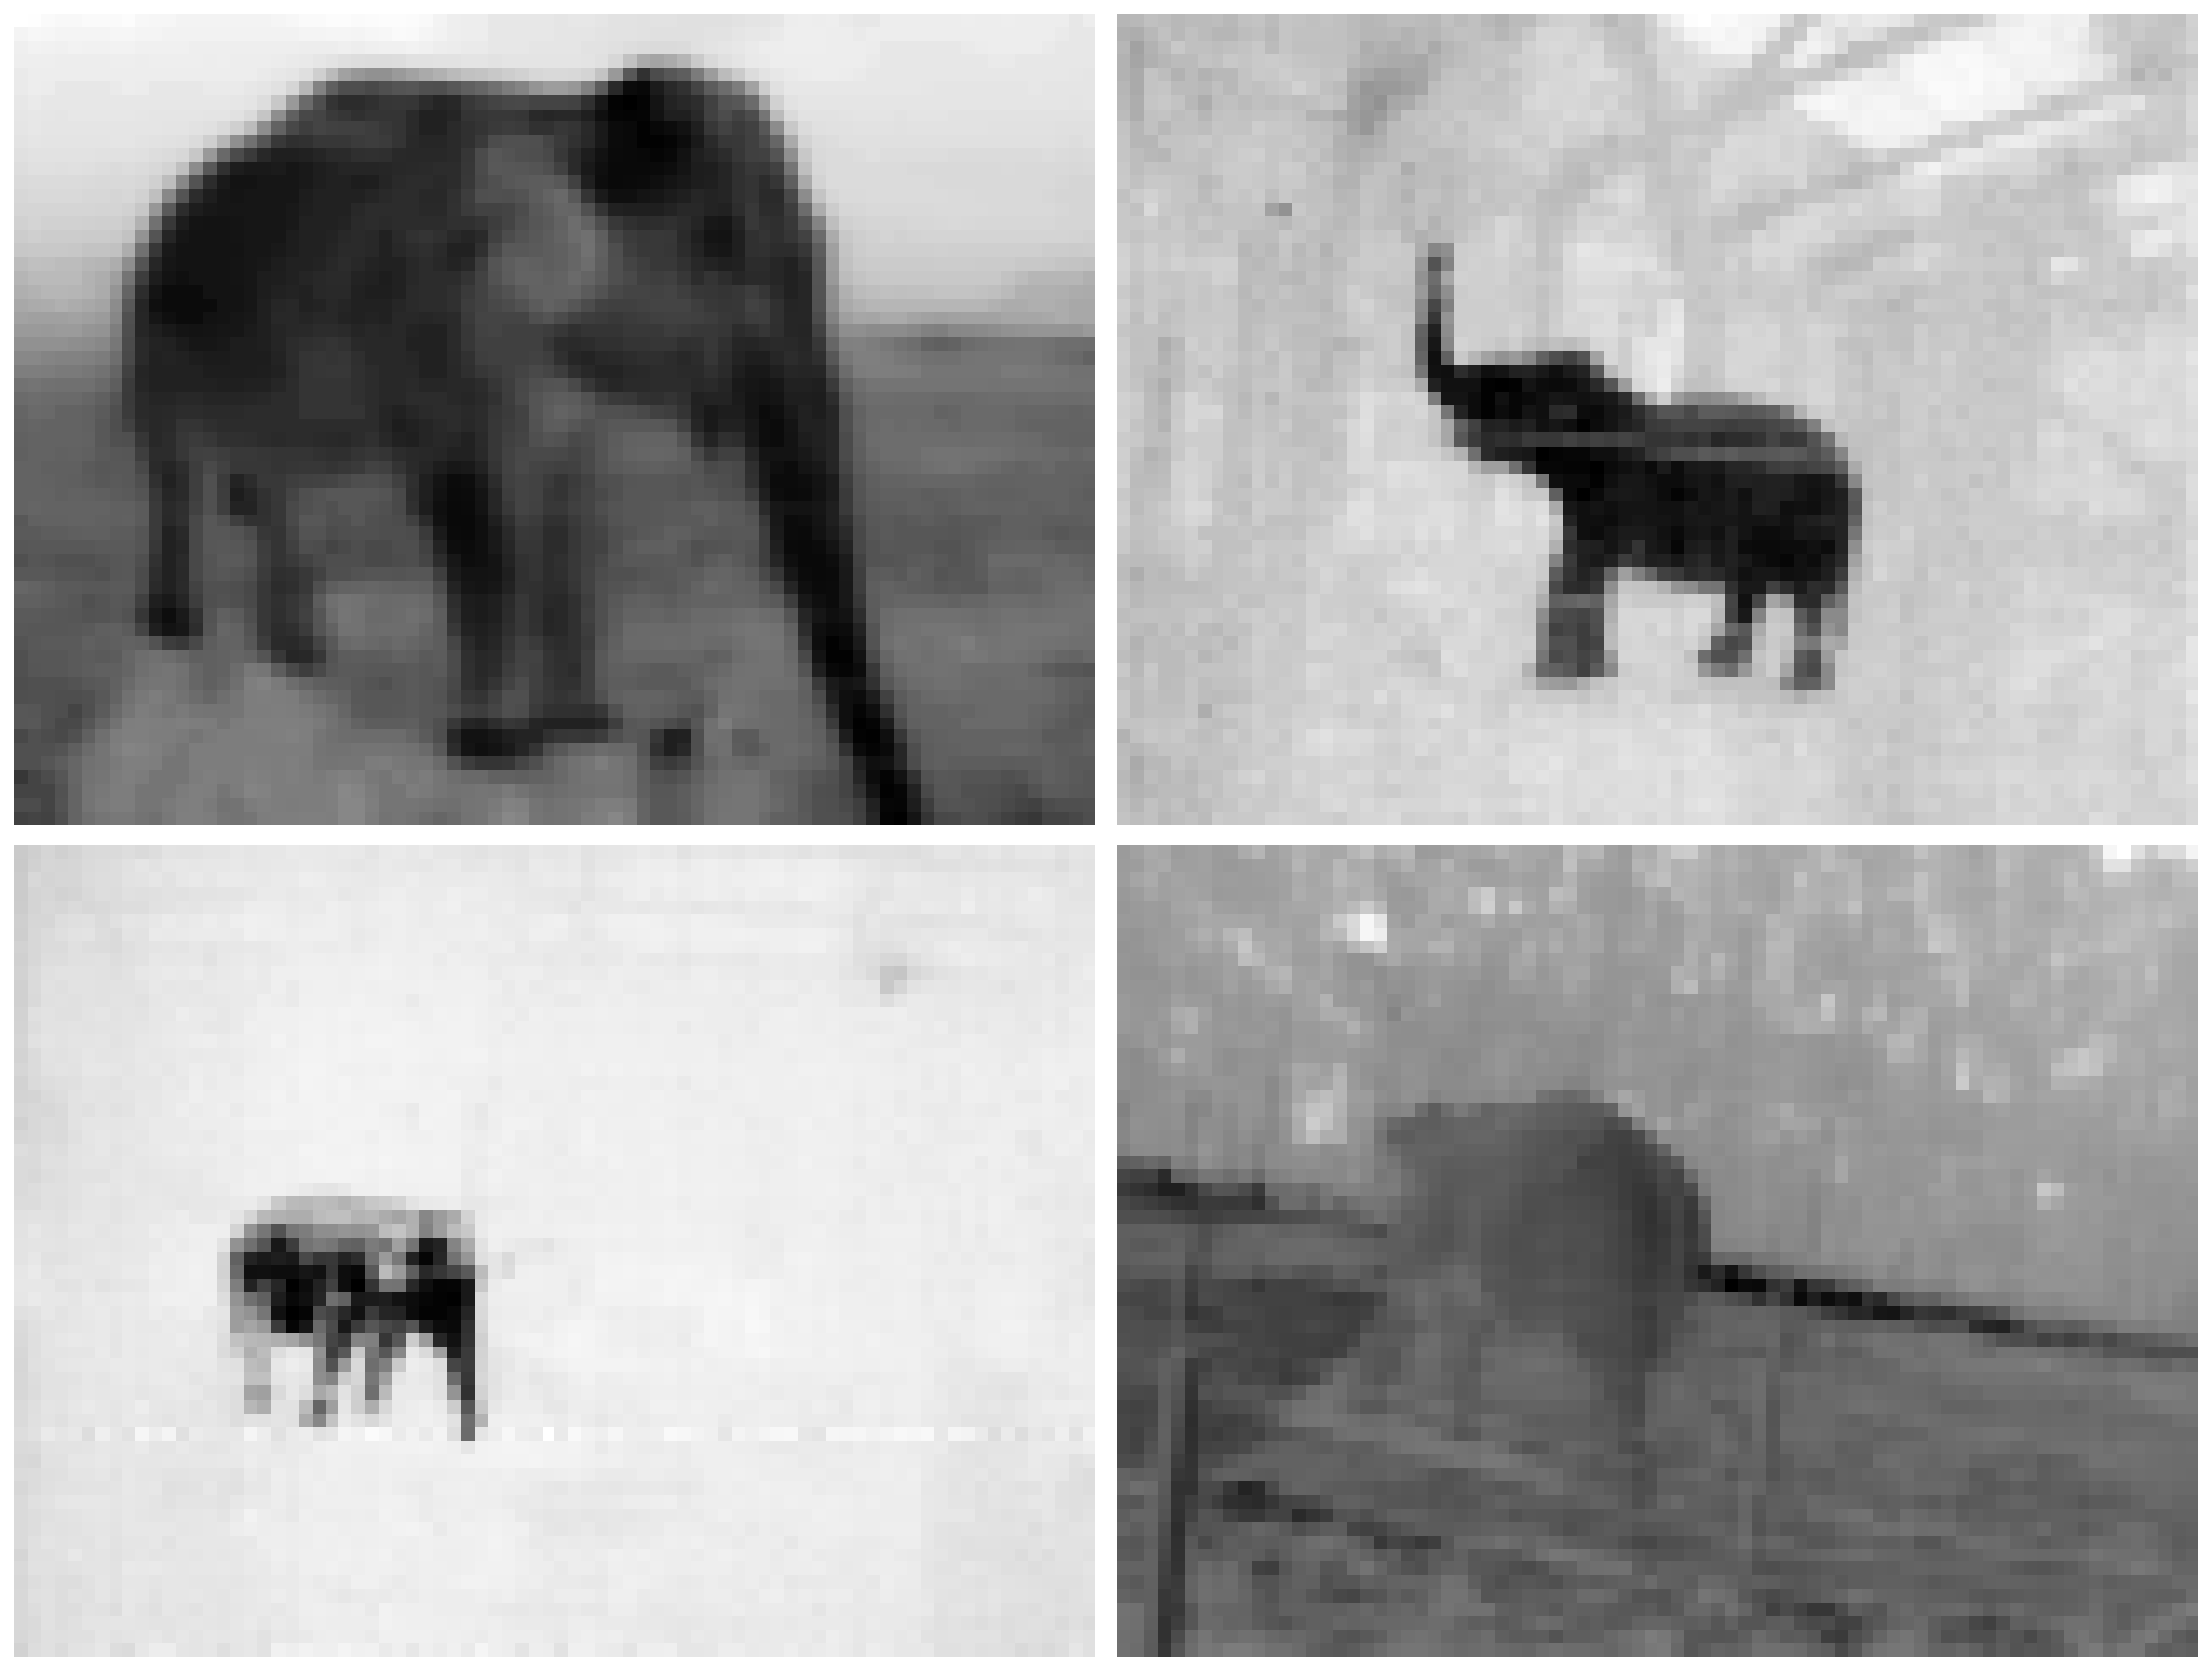
\includegraphics{four_elephants.pdf}}
    \caption{Thermal images of elephants from the dataset.}
    \label{four_elephants}
\end{figure}


A small part of the thermal image dataset was provided by us. This was done because the number of images of cows was low compared to the number of human and elephant images, and because we also did not have any images that could be used for the nature/random class.
We wanted to gather images as quickly and efficiently as possible, so we built a prototype camera made out of an FLIR Lepton 2.5 breakout board, a Raspberry Pi Zero, and a power bank.
We used an open-source library \cite{flir_github} for the FLIR Lepton module, which used a simple C program to take a single image with a thermal camera and save it to a Raspberry Pi.
The image of the setup can be seen in Figure \ref{cow_camera}.

\begin{figure}[ht]
    \centering
    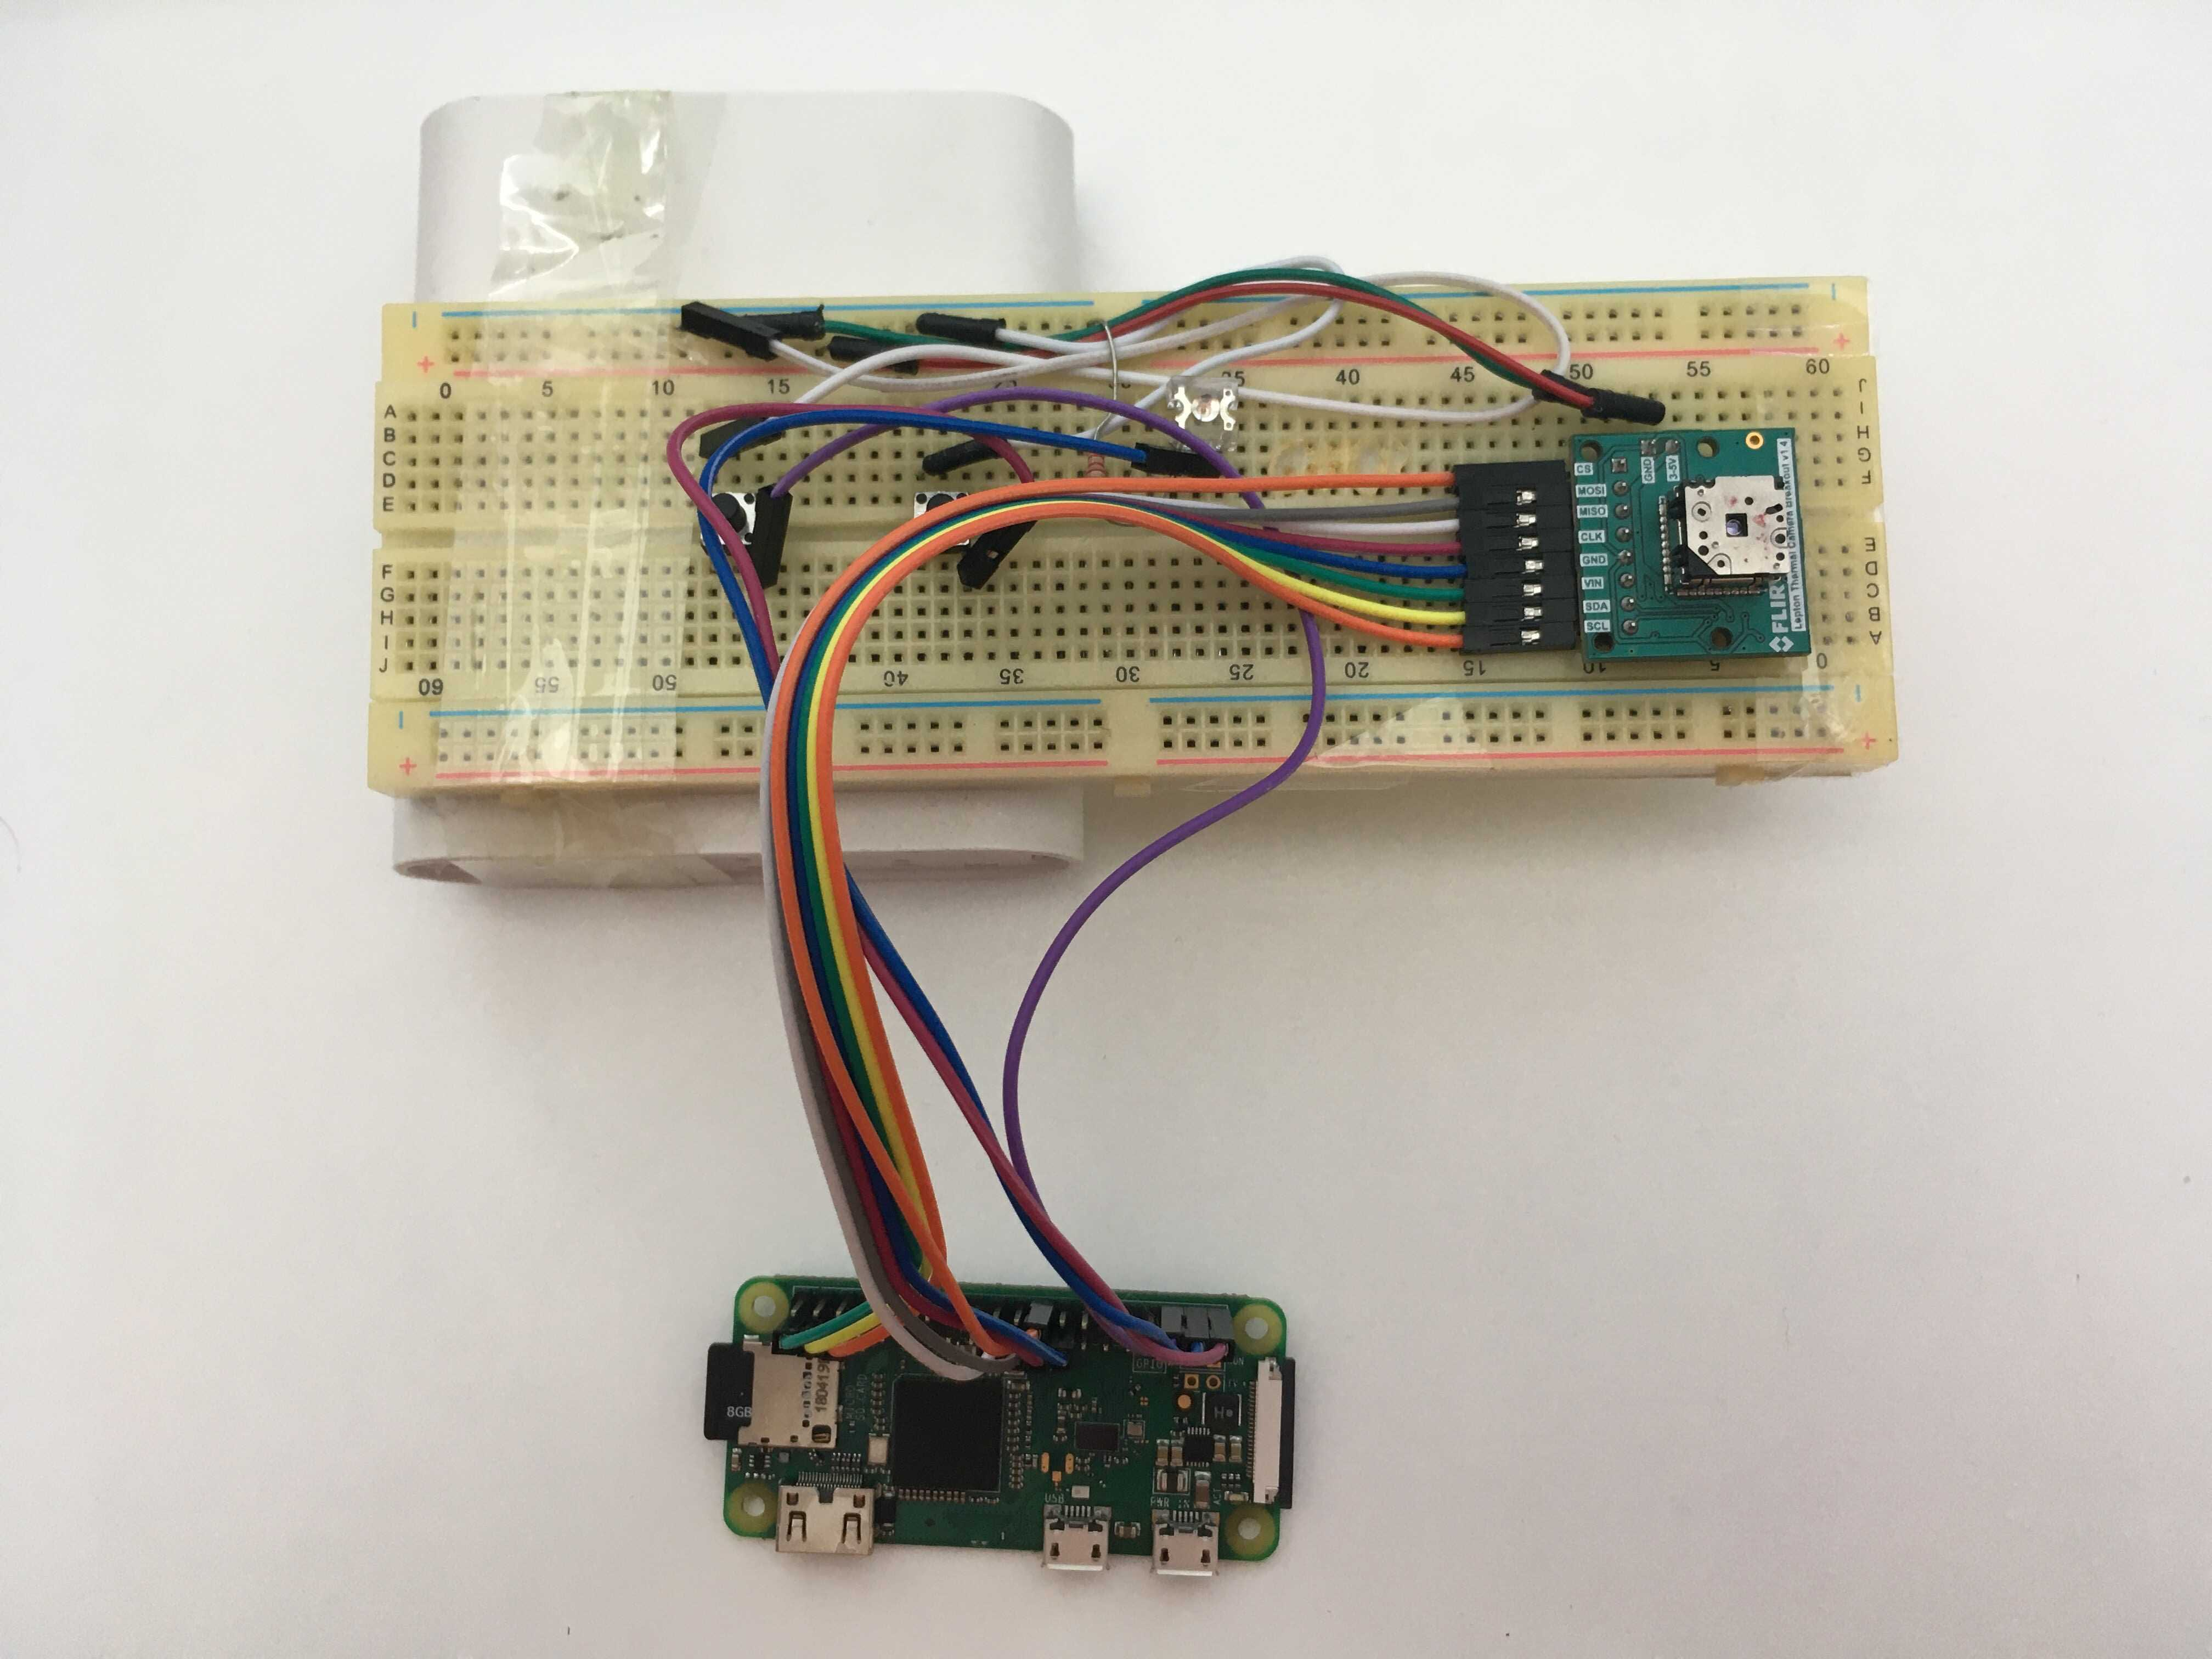
\includegraphics[width=1.0\linewidth]{cow_camera.jpg} 
    \caption{Camera setup used for taking thermal images with FLIR Lepton 2.5.}
    \label{cow_camera}
\end{figure}

We wrote a simple Python script that executed the C program every time we pressed the trigger push-button.
An additional shutdown button was added to call the Raspberry Pi shutdown routine, as removing power from it forcibly would corrupt freshly taken thermal images on the Raspberry Pi's SD card.

With this setup, we made 365 images of cows in varying conditions, 308 images of nature, and 124 images of humans that were made on the go.
We then sorted the images manually into appropriate folders and added them to the dataset.


\section{ Exploring the dataset} \label{exploring_dataset}

A thermal image dataset created by Arribada was given to us in the form of a Google Drive folder, which we downloaded to our computer. 

After examining the folder, we came to several conclusions.

\begin{enumerate}
    \item We saw that the primary focus of the Arribada team was to build an object localization model, not an image classification model.
In object localisation, the Neural Network draws bounding boxes around objects that it recognises and assigns them labels, while the image classification model only labels the image as a whole.
Object localization produces a bigger and more complex model than image classification, and it is unsuitable for running on a microcontroller.
All major work that was done by the Arribada team was contained in one folder where each image had an accompanying text file of the same name.
Text files were produced by a DeepLabel software, which is used for preparing images for training object localisation models.
Each line in a text file described the location of the bounding box and its label.
This dataset format was not suitable for us, as many images contained more bounding boxes, which would be troublesome to sort into a distinct label.

We later saw that there were a few folders with names such as "Human", "Single Elephant", "Multiple Separate Elephants", "Multiple obstructing Elephants", "Cows", "Goats" and so on, which contained sorted images that we could use.
We merged all folders with elephant pictures into one folder, as we did not care if the model can differentiate how many elephants are on a taken image, as we only wanted to know if there were any elephants on it or not.

    \item We found out that all images were documented in a large Excel database.
For each image, there was a row in a database that connected the image file name with the information on where the image was taken and with what sensor.
This enabled us to generate the graph seen in Figure \ref{nested_donut1}.

\begin{figure}[ht]
    \centering
    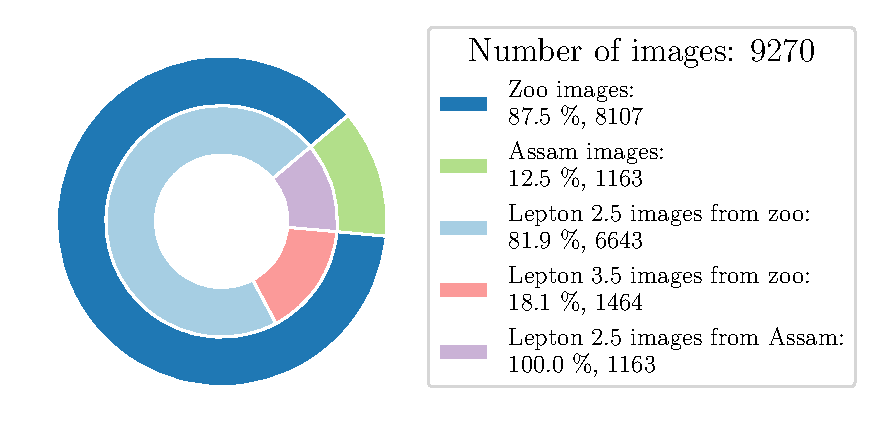
\includegraphics{nested_donut1.pdf} 
    \caption{Distribution of used images from thermal dataset depending on image location and type of sensor.}
    \label{nested_donut1}
\end{figure}

We used a total of 13,667 images from the thermal image dataset: almost 88 \% of them were made in Whipsnade Zoo, while the rest of them were made in Assam.
All images from Assam were made with the FLIR Lepton 2.5, while both cameras were used in Whipsnade zoo.However, more photos were made with the 2.5 version of the thermal camera.

    \item After inspecting the folder with goat images manually, we saw that it contained mostly images of a herd of goats standing around a single elephant.
This folder was usable only for object localisation ML models, where each goat could be tagged with a bounding box. 
In the case of an image classification model, this sort of training data is not desirable, as it would be too similar to another separate class, in our case the elephant class.
We therefore dropped goat images out of our training data entirely.
Livestock class was replaced with cow class.

    \item We also realised that there was a large class imbalance, as seen in Figure \ref{nested_donut2} in favour of the elephant class.

\begin{figure}[ht]
    \centering
    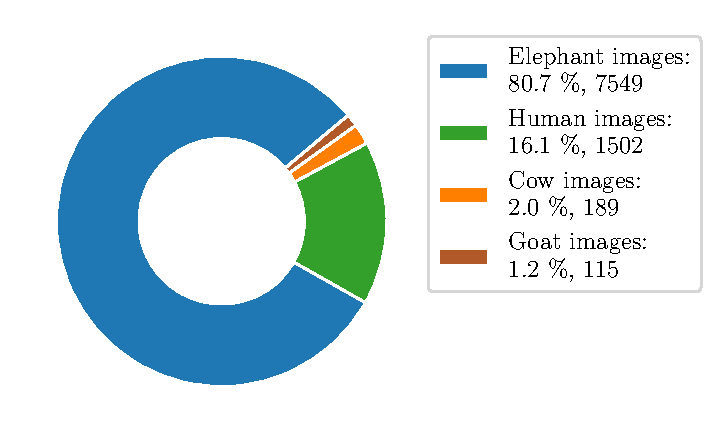
\includegraphics{nested_donut2.pdf} 
    \caption{Class distribution of thermal images.}
    \label{nested_donut2}
\end{figure}

The number of elephant images was more than 4 times larger than the number of images of the all other classes combined.
We solved this issue by acquiring more images of the minority class and oversampling the minority class.
\end{enumerate}


\section{ Image preprocessing}

The image preprocessing phase is a pipeline process that differs from project to project.
Our process can be seen in Figure \ref{image_preparation}.

\begin{figure}[ht]
    \centering
    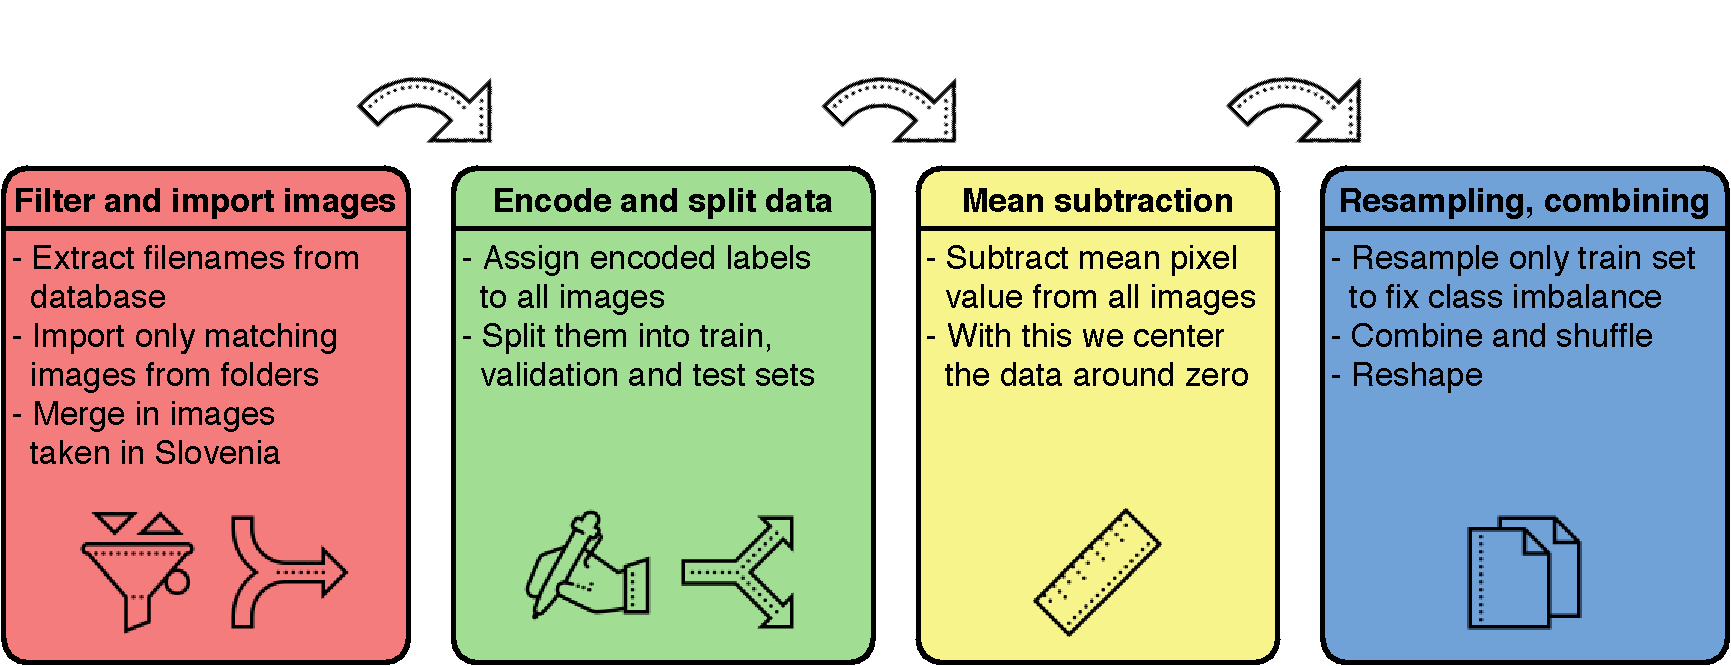
\includegraphics[width=1.0\linewidth]{image_preparation.pdf} 
    \caption[Image preprocessing pipeline.]{Image preprocessing pipeline. Icons source:\cite{icons}}
    \label{image_preparation}
\end{figure}

At the start of the process, we compared the filenames of each separate folder to the list of filenames found in the Excel database.
We imported only the images found in both sources, as lists were not identical, and we wanted to keep track of the different metadata information.
As some images were made with two different FLIR Lepton cameras with different resolutions (60 x 80 and 120 x 160), we downscaled higher resolution images directly in the importing process.
After this, we added images that were taken by us in Slovenia.
At this point, we had four separate Numpy arrays, one for each class, with 3 dimensions: The first dimension stored a number of different images in that class, the second and third dimensions stored images pixel values (60 and 80 pixels respectively).

The next step was assigning labels to each image.
As the output of NNs are numbers, we cannot just assign labels in strings format to data.
Instead, we assigned every image a single number that represented that class, 0 for an elephant, 1 for a human, 2 for a cow, and 3 for a nature/random class.
We shuffled images inside of each class and then split them into training, validation and test sets.

The training set was used for model training, while the validation set helped to choose the best model based on accuracy.
The test set is normally set aside and used only at the end, after the model is chosen, to assess how the model, performs on never seen data.
If we did not use the validation set and only chose the best model according to the test set, we would be overfitting a model and we would have no accurate measure of how well our model would perform on unseen data.

At end of this step we had 4 different Python dictionaries for each class.
Each dictionary had 3 key-value pairs for every training, validation, and test set, which held image data and encoded labels.

We next applied the simplest form of normalisation to all images, a mean subtraction.
We calculated a two-dimensional matrix that held mean values of pixels averaged over the whole training set, which we subtracted from all images, essentially zero centering the data.
This is a common preprocessing step in every ML image preprocessing pipeline, which is usually combined with standardisation\footnotemark.

\footnotetext{Standardisation scales the whole range of input pixel values into -1 and 1 interval.
This is only needed if different input values have widely different ranges\cite{cs231n}.
Because images that were created with the FLIR camera were all 8-bit encoded and therefore had the same range, this was not needed.}

We achieved this by resampling the human, cow, and nature/random classes.
The human class was resampled 5 times, while both cow and nature/random classes were resampled 8 times.
Figure \ref{resampled} shows the distribution of training images before and after resampling.

\begin{figure}[ht] 
    \begin{subfigure}[b]{1\textwidth}
        \centering
        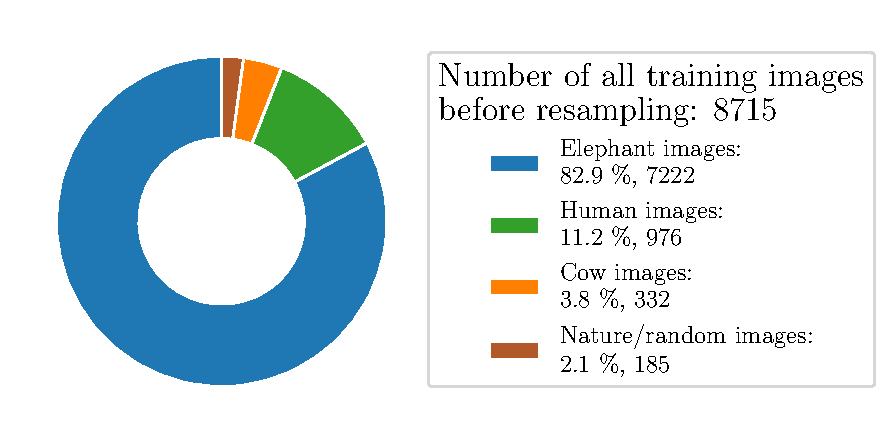
\includegraphics[width=1.0\linewidth]{nested_donut3.pdf} 
    \end{subfigure}
    \unskip\ \hrule\ 
    \begin{subfigure}[b]{1\textwidth}
        \centering
        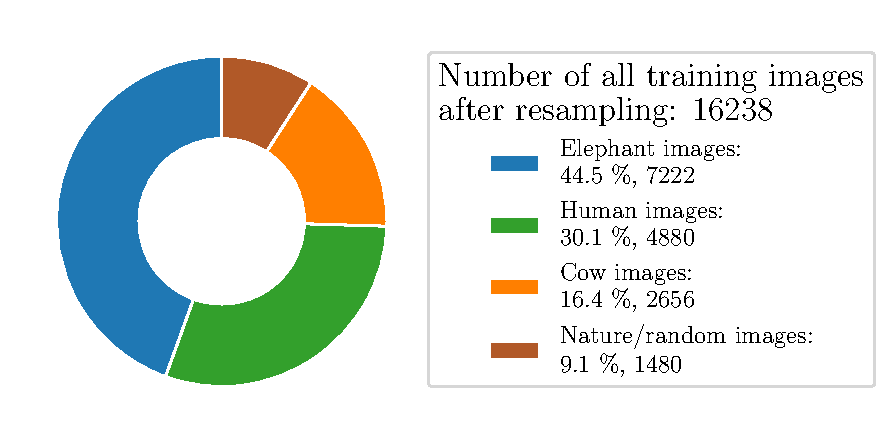
\includegraphics[width=1.0\linewidth]{nested_donut4.pdf} 
    \end{subfigure}
    
    \caption{ Distribution of training images before and after resampling.}
    \label{resampled}
\end{figure}

We only resampled training sets, not validation or test sets.
If we resampled everything, the model would be seeing the same image several times during testing, thus reporting incorrect accuracy in the validation and test phases.

After resampling we merged and shuffled all data, and saved it to the disk for later use.

\newpage
\section{ Model creation and training}\label{cnn_ref}

For the creation of CNN models, we used Keras Sequential API and a Keras Tuner module.
Sequential API abstracted many low-level details of the model's design.
While specifying layers, we only had to specify what type of layer we wanted, its size and layer-specific features. 
We did not have to keep track of any connections between or in layers, as this was done automatically by Keras.

For a model architecture we decided to use a simplified version of the common CNN architecture that was shown in Figure \ref{convnet}.
The best way to present the model is by inspecting the Sequential API code that creates it, and the code is shown in Figure \ref{model_code}.

The model consisted of two pairs of convolutional and max-pooling layers, followed by a final convolutional layer.
For activation the function ReLu was chosen, as it is currently the most effective and popular option\cite{cs231n}\cite{geron}.
The padding option was set to same, which meant that a spatial dimension of a volume would not change before and after a convolutional layer.
Pooling layer kernel size was set to 2 x 2, with a default stride of 2.

The output volume of the last convolutional layer was flattened out into a single vector and fed into a dense layer, which was followed by a dropout layer\footnotemark.

\footnotetext{ The Dropout layer decides with probability $p$ in each training step how many activations from the previous layer will be passed on to the next layer.
It is active only during the training phase, during the testing phase activations are multiplied with $(1-p)$ factor to compensate.
It is a very popular type of regularisation technique, which makes models more robust to the input data\cite{geron}.}

The last dense layer was a final output layer with only 4 neurons, each one representing one class.
Softmax activation was used to calculate class probabilities.
The model was set to use the Adam optimizer and Sparse Categorical Crossentropy loss function.
Adam is an upgraded version of the gradient descent method, which adapts the learning rate automatically to decaying gradients\cite{geron}.
It is generally easier to use than gradient descent, as it requires less tuning or learning rate hyperparameters.
Sparse Categorical Crossentropy loss function is used when building a multi-class classifier.

The above set hyperparameters follow the general rules of thumb and serve as a good starting point when building CNNs\cite{cs231n}.
However, hyperparameters such as the number of filters, filter size, size of a hidden dense layer, dropout rate, and learning rate, are specific to each dataset, and cannot be chosen heuristically.

To find hyperparameters that would yield the highest accuracy we used the Keras Tuner module.
The exact configuration of a Keras Tuner module and comparison of trained models is presented and discussed in Section \ref{model_comparisons}.

\lstset{style=mystyle}
\begin{figure}[ht] 
    \begin{lstlisting}[language=Python]
        model = models.Sequential()

        model.add(Conv2D(FilterNum1, FilterSize, 
                         activation='relu', 
                         padding="same", 
                         input_shape=(60,80, 1)))

        model.add(MaxPooling2D((2, 2)))

        model.add(Conv2D(FilterNum2, FilterSize, 
                         activation='relu', 
                         padding="same")

        model.add(MaxPooling2D((2, 2)))

        model.add(Conv2D(FilterNum3, FilterSize, 
                         activation='relu', 
                         padding="same")

        model.add(Flatten())

        model.add(Dense(DenseSize, activation='relu'))
        model.add(Dropout(DropoutRate))
        model.add(Dense(4), activation='softmax')
    \end{lstlisting}
    \caption{ CNN architecture written in Python using Keras Sequential API.}
    \label{model_code}
\end{figure}


\section{ Model optimisation}

Keras supports saving models in h5 format, which model's architecture, values of weights, and information used while compiling the model.
h5 format cannot be used directly for running trained models on mobile devices and microcontrollers: conversion to a .tflite format has to be done with the TFLite Converter tool.

The TFLite converter can convert a model in .h5 format into four differently optimised tflite models:
\begin{itemize}
    \item \textbf{Non-quantized tflite model,} no quantization, just basic conversion from .h5 to .tflite format is done.
    \item \textbf{Float16 model,} weights are quantized from 32-bit to 16-bit floating-point values. The model size is split in half, and the accuracy decrease is minimal, but there is no boost in execution speed.
    \item \textbf{Dynamic model,} weights are quantized as 8-bit values, but operations are still done in floating-point math. Models are 4 times smaller and execution speed is faster when compared to float16 optimisation but slower than full integer optimisation.
    \item \textbf{Full integer model,} weights, biases, and math operations are quantized, execution speed is increased. It requires a representative dataset at conversion time.
\end{itemize}

A full integer model is an ideal choice for running models on microcontrollers, although, it should be noted that not all operations have full integer math support in TFLite Micro.

Furthermore, created tflite models need to be converted into a format that is understandable to the C++ TFlite API running on a microcontroller.
This is done with the \textbf{xxd}, a Linux command-line tool that creates a hex dump out of any input file.
By setting \verb|-i| flag, the xxd tool creates a hex dump of our model,and formats it as a char array in the C programming language. 

To automate the optimisation process we wrote a Python script that took the model in raw .h5 format and converted it into every possible version of the optimised tflite model.
Each model was then processed with the xxd tool and pairs of .c and .h files were created, ready to be included in our application code.


\section{ Neural Network model design in Edge Impulse Studio}

Designing a Neural Network with Edge Impulse is a much less involved process than the one we described above, because many steps of image preprocessing are automated.
To start with NN design, we first had to upload our image data to the Edge Impulse Studio project.
This can be done either by connecting an S3 bucket\footnotemark with data with the Edge Impulse account, and transferring data to a specific project or by using the Edge Impulse command-line tools to upload image data from a computer directly to a project.
We chose the S3 bucket approach, as once the data was uploaded it was trivial to transfer it to different projects.

\footnotetext{Simple Storage Service or S3 is another service provided by Amazon, used for storing a large amount of data in the cloud.}

After the data were uploaded, the rest of the NN design was done through the Edge Impulse web interface.
In Figure \ref{edge_impulse_screenshot} we can see the so-called Impulse Design tab, where we design a Neural Network by choosing different blocks.
With input blocks, we tell what kind of data are we inputting, either image or time-series data, and with processing blocks we decide how are we going to extract features.
Input and preprocessing blocks always return same output given the same input, while learning blocks are trainable and learn from previous experiences.
For learning block, we can choose to use a Neural Network provided by Keras, an anomaly detection algorithm, or a pre-trained model for transfer learning.

\begin{figure}[ht]
    \centering
    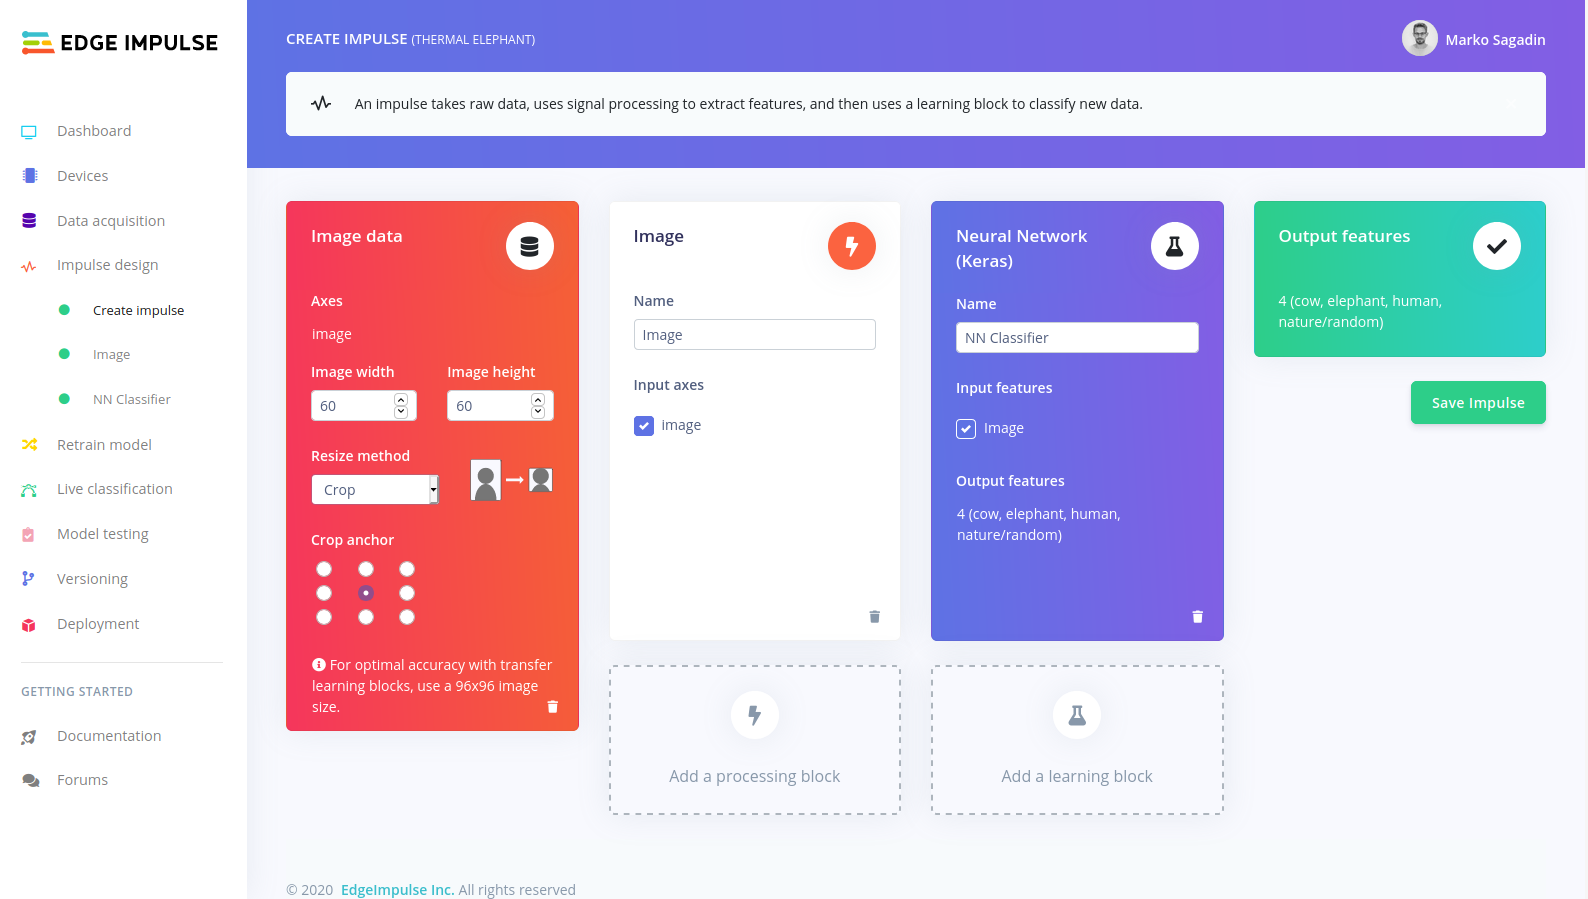
\includegraphics[width=1.0\linewidth]{edge_impulse_screenshot.png} 
    \caption{Creating a Neural Network in Edge Impulse Studio.}
    \label{edge_impulse_screenshot}
\end{figure}

Since we were training with image data, we selected an image input block. As Edge Impulse did not support images of different image ratios at the time, we had to crop our images to 60 x 60 pixels.
For the processing block, we selected the image processing block as this was the only possible choice.
For the learning block we were using both Keras's Neural Network block and Transfer Learning block.

Both of the blocks are configurable.
We could either define our network with different blocks representing layers, or switch to the text editor with Keras Sequential API code, where we could make our adjustments.
Settings such as learning rate, number of epochs, and confidence rating are also available, regardless of the option we chose.
Training of Neural Networks inside Edge Impulse Studio is done in a cloud, so as users we do not have to worry about setting up a development environment.
We only have to start it and wait for it to finish.

After training was done, Edge Impulse showed how well the model was performing on the validation data, how much flash and RAM would it need, and approximately how long on-device inference would take, based on the frequency and the processor of the microcontroller.

An example of the output is presented in Figure \ref{edge_impulse_screenshot2}, where inferencing time is estimated for a Cortex-M4 microcontroller, running at 80 \si{\mega\hertz}.
Edge Impulse also does the conversion to an optimised full-integer model automatically.

\begin{figure}[ht]
    \centering
    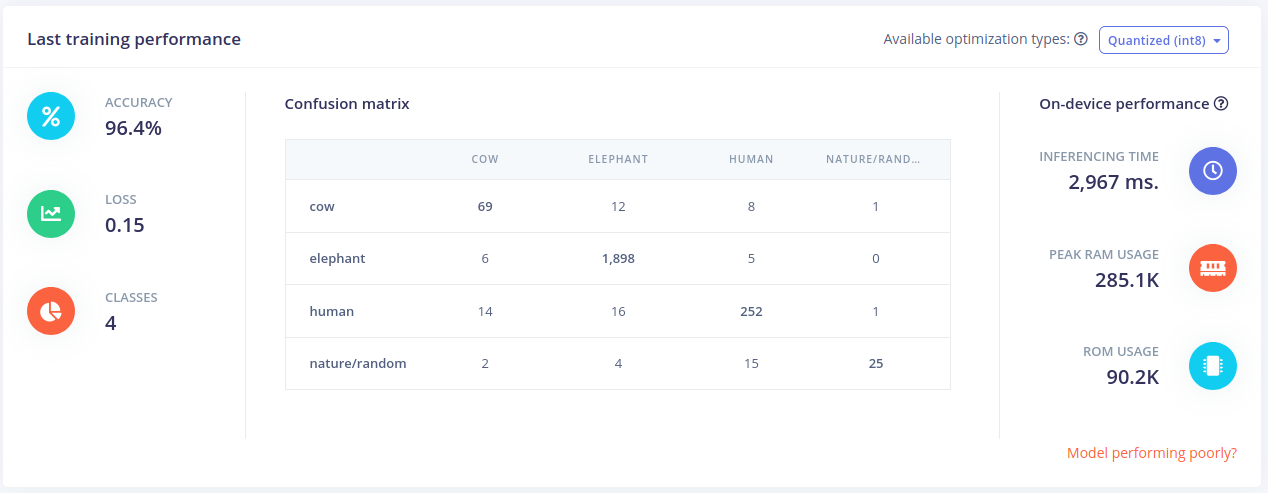
\includegraphics[width=1.0\linewidth]{edge_impulse_screenshot2.png} 
    \caption{ Training performance report.}
    \label{edge_impulse_screenshot2}
\end{figure}

The final step was deploying the trained model to the microcontroller.
This step is fairly simple, as Edge Impulse provides a few example projects on their GitHub for the different platforms that it supports.
As we wanted to compare the performance of the models on STM32f767ZI, we chose the Mbed platform.
We copied the example Mbed project from GitHub, and in the Edge Impulse Studio we selected to generate an inferencing library with our model for the Mbed platform.
We extracted the library, which consisted of C++ files, into an example project and compiled it.
An example project just runs the inference continuously on one image and outputs results over the serial port.
A performance comparison between this example project and our implementation is done in Section TODO ADD REFERENCE.
